%

\chapter{基于枝干合并的轻量化处理}
\label{cha:branchcombine}
用基于多方向迭代与步长探索得到的三维树木骨架通常是很细致和准确的,尽管它相对于
用3DSMAX等建模工具手工建模得到的面片模型已经大大的轻量化了。但是如果应用是用于
大规模的树木建模,那么我们有必要根据应用需求进一步进行轻量化处理。

\section{L-System的尝试}
\label{subsec:lsystem}

\subsection{L-System简介}
L-System是一种并行的重写系统和正规语法,
它的结构可以用可以定义为一个3元组:\\
\[\mathbf{M} = (V, \omega, P)\]
其中:\\
\begin{itemize}
	\item $\mathbf{V}$(字母表) 表示可以被替代的字符的集合。
	\item $\mathbf{\omega}$(初始串) 表示L-System的初始状态。
	\item $\mathbf{P}$(规则集合) 表示一系列的衍生规则。
\end{itemize}
L-System可以根据这三个组成部分的不同而递归地产生形态各异的字符串。
由于L-System具有递归生长的特性,因此我们可以用L-System规则来表达一个具有自相似形态
或者分形结构的物体,比如本文所研究的对象\raisebox{0.5mm}{------}树木。

\subsection{树木模型的参数化L-System规则抽取}
球面海龟几何的提出,用参数化的L-System规则描述了树木的结构信息。在球面海龟几何中,
节点的空间几何信息用4个量(长度$l$、半径$r$、父子枝夹角$\theta$和水平转角$\phi$)
和4个扩展符号(+、-、\&、$\wedge$)来表示:
\begin{itemize}
	\item $+(l)$	表示以当前位置为起点,在当前方向上前进$l$单位个长度
	\item $!(r)$	表示设置当前节点半径为$r$
	\item $\&(\theta)$	表示设置父子枝夹角为$\theta$
	\item $\wedge(\phi)$	设置水平偏角为$\phi$
\end{itemize}
在球面海龟几何中,将每个骨架节点生成一条参数化的L-System规则,形如:\\
\begin{equation} \label{eq:turtle}
N(l,r) \rightarrow \&(\theta_0)\wedge(\phi_0)!(r) + (l)S_0(l*a_0,r*b_0)...\&(\theta_n)\wedge(\phi_n)!(r) + (l)S_n(l*a_n,r*b_n)
\end{equation}

其中N表示当前枝条,$S_0~S_n$表示当前枝条的n个子枝条,$a_i和b_i$分别表示第i个子枝条
与当前枝条的长度比和半径比,$\theta_i和\phi_i$分别表示第i个子枝条与当前枝条的空间
夹角和水平偏角。

\subsection{使用L-System进行树木轻量化建模遇到的问题}
在用参数化L-System进行树木轻量化建模时,在进行规则归纳时,有个难以克服的问题。考虑
将规则\ref{eq:turtle}中的$a_0$换成$a_0'$,则规则变成一个完全不同的规则。这意味着对于
两个分支规则,这两个规则中的子枝的长度,半径,转交,偏角等必须完全相等才能归纳为同
一个规则。而对于自然界中形态结构复杂的树木,每个分支规则几乎不可能完全等同于另一个
规则。

对上面的问题有一种解决方法就是将参数区间化,将属于同一区间的参数的值视为相同。比如
我们可以将父子枝间的转角分为18个区间,每个区间的大小为10度。但是经过分析就可以察觉,
这并没有从根本上解决这个问题。假设我们将这4个变量都各自划分为10个区间,那么规则总数
最多可以有10000个,而且在这种情况下,两个规律相同的几率也是非常小的。如果我们将分区
数量减少,则又有可能将本来差异比较大的规则归纳为一个规则,不符合真实感的要求。

所以,经过分析,这种用参数化L-System进行树木轻量化建模的方法并不适用于从骨架中去抽取
规则,而是适用于反向地用其描述的规则去产生一棵树,如台湾学者戴文凯就对单棵树的L-System
规则进行随机扰动而轻量化的建模出了整片森林。

\section{基于枝干合并的树木分级轻量化}
\label{subsec:branchmerge}
用L-System的方法抽取规则所产生的问题,从本质上看,是由于自然界中的树木形态太复杂和多变。
与其从一个本就不规则生长的事物中去抽取规则,还不如直接地在其逻辑结构上进行一系列的轻量
化操作。本文提出了分级化地对已抽取的树木骨架中对视觉影响不大的部分进行合并的方法,从而在尽可能
保证模型的视觉效果的基础上,进一步地减小树木模型的体积,使得其能更广泛地应用到WebVR、WebGame
等各个领域。

树枝的结构其实只由核心的一些枝干组成,其他的枝干只是对其结构进行微调。所以在要求进一步轻量化
的前提下,本文提出了分别从纵向和横向对树枝进行合并的方法,以去掉一些只是起到微调作用的枝干。
这种方法在尽可能保证真实感不过多丢失的前提下对树枝进行简化操作,以适应更广泛的Web应用领域。

\subsection{基于夹角的枝干纵向合并算法}

纵向合并表示从父到子,从根到页进行纵向递归式的合并。若当前节点与其父节点和子节点的夹角小于所设定
的阈值,那么则将该节点去掉,并将其子节点连接到其父节点。注意,若该节点的子节点数目不只一个,
那么我们不对它进行合并操作,因为将该节点的所有子节点加到该节点的父节点上去有违真实感。
图\ref{fig:vert}展示了树枝纵向合并过程。图\ref{fig:vert}(a)为输入的树枝骨架,并且当前节点
为\textbf{B},其父节点为\textbf{A},且只有唯一的子节点\textbf{C}。设合并角度阈值为$\alpha$,
假设\textbf{AB,BC}之间的夹角b小于合并阈值$\alpha$,那么将\textbf{B}剔除,并将\textbf{C}作为
\textbf{A}的子节点。同理,在图\ref{fig:vert}(b)中,若夹角c小于阈值$\alpha$,那么也将\textbf{AC}
和\textbf{CD}合并。在图\ref{fig:vert}(c)中,由于节点\textbf{D}有两个孩子,所以不对其进行合并
操作。

基于夹角的枝干纵向合并算法的伪代码在算法\ref{alg:vertical}中给出。

\begin{figure}[H]
	\centering
	\subfloat[合并AB、BC]{
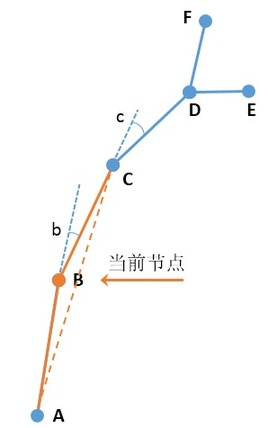
\includegraphics[height=5cm]{vert1.jpg}}
\hspace{4em}
	\subfloat[合并AC、CD]{
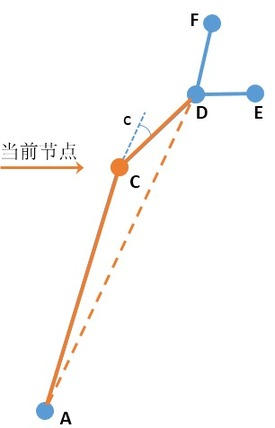
\includegraphics[height=5cm]{vert2.jpg}}
\hspace{4em}
	\subfloat[合并完成]{
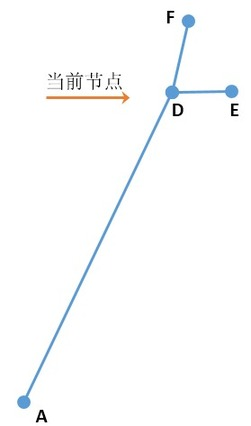
\includegraphics[height=5cm]{vert3.jpg}}
	\caption{树枝简化过程}
	\label{fig:vert}
\end{figure}

\begin{algorithm}[H]
	\caption{基于夹角的枝干纵向合并}
	\label{alg:vertical}
	\begin{algorithmic}[1] 
		%\Comment {根据纵向合并角度参数,以当前节点为发起点递归式地纵向合并枝干}
		\Require 纵向合并角度$\alpha$
		\Require 当前节点$N$
		\Ensure None
		\ForAll{节点$N'\in N.Children$}
		\While{$N'.ChildCount = 1$}
		\State $\vec{u} \gets N'.Position-N.Position$
		\State $\vec{v} \gets N''.Position-N'.Position$
		\State $\gamma \gets \cos^{-1}({\frac{\vec{u} \cdot \vec{v}}{|\vec{u}|\cdot|\vec{v}|}})$
		\If{$\gamma<\alpha$}
		\State $N.child \gets N.AddChild(N'')$
		\State $N.child \gets N.DeleteChild(N') $
		\EndIf
		\State $N' \gets N'.FirstChild$
		\EndWhile
		\EndFor
		\If{$N.ChildCount > 1$}
		\ForAll{节点$N'\in N.Children$}
		\State 以$N'$为当前节点递归调用该函数
		\EndFor
		\EndIf
	\end{algorithmic}
\end{algorithm}

\subsection{基于端点距离的枝干横向合并算法}

横向合并指的是对非常靠近的叶子节点进行合并。之所以只对叶子节点进行合并,是
因为非叶子节点下面都有若干棵子树,若对它们进行合并,必须对它们下面的子树也进行合并。而合并子树
显然就使得真实感下降很大,因为这不只是局部微调,而是若干子树的变动。对于横向合并,不再是使用角度
来衡量两个子枝的靠近程度,而是使用子节点间的欧式距离来表示,因为合并两个角度相差小但是长度相差大的
子枝也会导致真实感的大幅下降。横向合并的伪代码在算法\ref{alg:hori}中
给出。

\begin{algorithm}[H]
	\caption{基于端点距离的枝干横向合并}
	\label{alg:hori}
	\begin{algorithmic}[1] 
	\Require 初始化横向合并距离阈值$\mu$
	\Require 设定当前节点$N$
	\Ensure None
	\ForAll{节点对$P\in N.Children$}
		\State $N_1 \gets P.FirstNode$
		\State $N_2 \gets P.SecondNode$
		\If{$N_1.ChildCount = 0 \wedge N_2.ChildCount = 0$}
		\State $\mathbf{\vec{u}} \gets N_1.Position$
		\State $\mathbf{\vec{v}} \gets N_2.Position$
		\State $\gamma \gets |\mathbf{\vec{u}} - \mathbf{\vec{u}}|$
			\If{$\gamma<\mu$}
				\State $New\ Node\ N'$
				\State $N'.Position \gets (N_1.Position+N_2.Position)/2$
				\State $N'.Radius \gets max(N_1.Radius,N_2.Radius)$
				\State $N.child \gets N.DeleteChild(N_1)$
				\State $N.child \gets N.DeleteChild(N_2)$
				\State $N.child \gets N.AddChild(N')$
				\State 退出循环并以当前节点N重新调用该函数
			\EndIf
		\EndIf
	\EndFor
	\ForAll{节点$P\in N.Children$}
		\State 以P为当前节点递归调用该函数
	\EndFor
\end{algorithmic}
\end{algorithm}

\subsection{综合使用横纵向合并}

纵向合并和横向合并单独使用时都具有很大的局限性,因为纵向合并只能对具有单个孩子并且没有
兄弟的节点进行纵向递归地调用,而横向合并又只能对叶子节点进行兄弟级别的合并。但是将两种
合并方法联合使用,将可以从整体上对树木进行微调操作,图\ref{fig:combine}对这一想法进行了
演示。\ref{fig:combine}(a)中经过纵向的\textbf{AB,BC}合并得到\ref{fig:combine}(b)。
\ref{fig:combine}(b)中由于\textbf{C}有两个子节点,无法进行纵向合并,所以考虑进行横向
合并\textbf{CD,CE},并得到\ref{fig:combine}(c)。最后进行一次纵向合并得到\ref{fig:combine}(d)。

\begin{figure}[H]
	\centering
	\subfloat[纵向合并AB,BC]{
	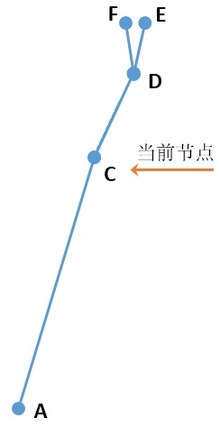
\includegraphics[height=6cm]{comb1.jpg}}
	\hspace{6em}
	\subfloat[横向合并CD,CE]{
	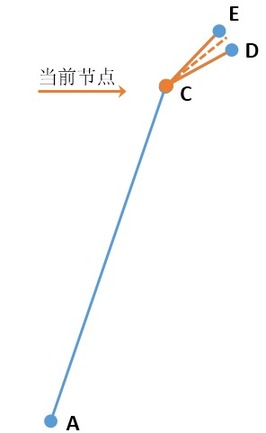
\includegraphics[height=6cm]{comb2.jpg}}
	\hspace{6em}
	\subfloat[纵向合并AC,CE]{
	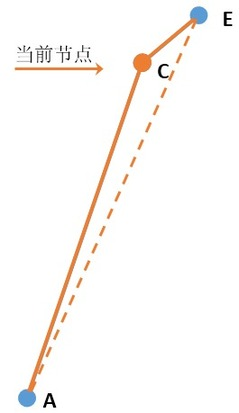
\includegraphics[height=6cm]{comb3.jpg}}
	\hspace{6em}
	\subfloat[合并完成]{
	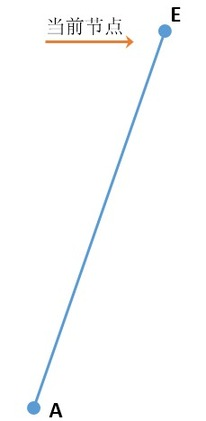
\includegraphics[height=6cm]{comb4.jpg}}
	\caption{联合使用纵向和横向合并}
	\label{fig:combine}
\end{figure}

\section{本章小节}
在得到骨架结构后,为了迎合轻量化的应用,本文对其进行轻量化操作。本章首先对传统的轻量化方法L-System进行了尝试,运用参数化
的L-System规则进行规则抽取,但是由于现实中树木的复杂性与不规则性,抽取出来的规则太多,以至于违背了轻量化的原则。于是本文
提出了基于枝干合并的轻量化方法,分别从纵向和横向对树木枝干进行合并,并对这两种方法进行有机的组合使用,以达到轻量化的目标。
